\documentclass[border=2pt]{standalone}
\usepackage{tikz}
\usepackage{amsmath}
\usepackage{mathtools}
\usepackage{adjustbox}
\usetikzlibrary{patterns}
\usetikzlibrary{calc} \usetikzlibrary{positioning} \usetikzlibrary{shapes,arrows} \usetikzlibrary{plotmarks}
\usetikzlibrary{positioning,decorations.pathreplacing}

\begin{document}

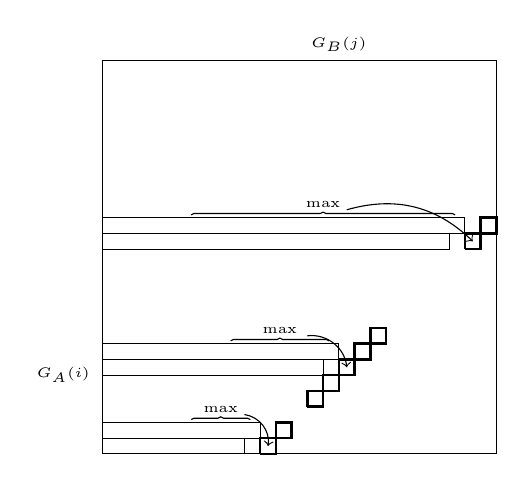
\begin{tikzpicture}

% table rectangle
\draw (0,0) -- (5,0) -- (5,5) -- (0,5) -- (0,0);
% rectangle: query dp[i][j]
\draw[line width=0.3mm] (3,1) -- (3.2,1) -- (3.2,1.2) -- (3,1.2) -- (3,1);

\node[] at (-0.5, 1) {\tiny $G_A(i)$};
\node[] at (3, 5.2) {\tiny $G_B(j)$};

% rectangle: range maximum for dp[i][j]
%\draw[line width=0.5mm, densely dotted] (1.5, 1.2) -- (3,1.2) -- (3, 4) -- (1.5, 4) -- (1.5, 1.2);


% begin wave
\draw[line width=0.3mm] (2.8,0.8) -- (3.0,0.8) -- (3.0,1.0) -- (2.8,1.0) -- (2.8,0.8);
\draw[line width=0.3mm] (2.6,0.6) -- (2.8,0.6) -- (2.8,0.8) -- (2.6,0.8) -- (2.6,0.6);

% mid wave
\draw[line width=0.3mm] (2.2,0.2) -- (2.4,0.2) -- (2.4,0.4) -- (2.2,0.4) -- (2.2,0.2);
\draw[line width=0.3mm] (2.0,0.0) -- (2.2,0.0) -- (2.2,0.2) -- (2.0,0.2) -- (2.0,0.0);
\draw[line width=0.3mm] (3.2,1.2) -- (3.4,1.2) -- (3.4,1.4) -- (3.2,1.4) -- (3.2,1.2);
\draw[line width=0.3mm] (3.4,1.4) -- (3.6,1.4) -- (3.6,1.6) -- (3.4,1.6) -- (3.4,1.4);

% end wave
\draw[line width=0.3mm] (4.6,2.6) -- (4.8,2.6) -- (4.8,2.8) -- (4.6,2.8) -- (4.6,2.6);
\draw[line width=0.3mm] (4.8,2.8) -- (5.0,2.8) -- (5.0,3.0) -- (4.8,3.0) -- (4.8,2.8);

% mid horizontal 
\draw (0.0, 1.4) -- (3.0, 1.4) -- (3.0, 1.2) -- (0.0, 1.2);
\draw (0.0, 1.2) -- (2.8, 1.2) -- (2.8, 1.0) -- (0.0, 1.0);

% begin horizontal 
\draw (0.0, 0.4) -- (2.0, 0.4) -- (2.0, 0.2) -- (0.0, 0.2);
\draw (0.0, 0.2) -- (1.8, 0.2) -- (1.8, 0.0) -- (0.0, 0.0);

% end horizontal 
\draw (0.0, 2.8) -- (4.4, 2.8) -- (4.4, 2.6) -- (0.0, 2.6);
\draw (0.0, 3.0) -- (4.6, 3.0) -- (4.6, 2.8) -- (0.0, 2.8);

\begin{scope}
\node[](start) at (1.5, 1.4) {};
\node[](end) at (3, 1.4) {};
\draw[decorate,decoration={brace,amplitude=1pt, raise=1pt}](start)--node[black,midway,above=0pt] {\tiny max}(end);
\path[solid,->](2.6, 1.5) edge [bend left=45]  (3.1, 1.1);
\end{scope}

\begin{scope}
\node[](start) at (1.0, 0.4) {};
\node[](end) at (2.0, 0.4) {};
\draw[decorate,decoration={brace,amplitude=1pt, raise=1pt}](start)--node[black,midway,above=0pt] {\tiny max}(end);
\path[solid,->](1.8, 0.5) edge [bend left=45]  (2.1, 0.1);
\end{scope}

\begin{scope}
\node[](start) at (1.0, 3.0) {};
\node[](end) at (4.6, 3.0) {};
\draw[decorate,decoration={brace,amplitude=1pt, raise=1pt}](start)--node[black,midway,above=0pt] {\tiny max}(end);
\path[solid,->](3.1, 3.1) edge [bend left=30]  (4.7, 2.7);
\end{scope}

\end{tikzpicture}

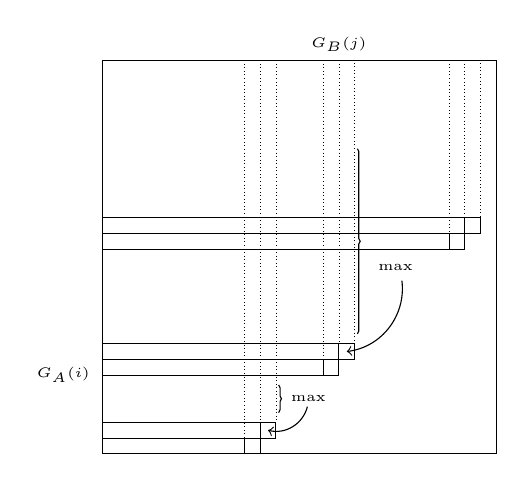
\begin{tikzpicture}

% table rectangle
\draw (0,0) -- (5,0) -- (5,5) -- (0,5) -- (0,0);
% rectangle: query dp[i][j]
\draw (2.8,1) -- (3,1) -- (3,1.2) -- (2.8,1.2) -- (2.8,1);

\node[] at (-0.5, 1) {\tiny $G_A(i)$};
\node[] at (3, 5.2) {\tiny $G_B(j)$};

% rectangle: range maximum for dp[i][j]
%\draw[line width=0.5mm, densely dotted] (1.5, 1.2) -- (3,1.2) -- (3, 4) -- (1.5, 4) -- (1.5, 1.2);


% begin wave
\draw (2.0,0.2) -- (2.2,0.2) -- (2.2,0.4) -- (2.0,0.4) -- (2.0,0.2);
\draw (1.8,0.0) -- (2.0,0.0) -- (2.0,0.2) -- (1.8,0.2) -- (1.8,0.0);

% mid wave
\draw (3.0,1.2) -- (3.2,1.2) -- (3.2,1.4) -- (3.0,1.4) -- (3.0,1.2);

% end wave
\draw (4.6,3.0) -- (4.8,3.0) -- (4.8,2.8) -- (4.6,2.8) -- (4.6,3.0);
\draw (4.4,2.8) -- (4.6,2.8) -- (4.6,2.6) -- (4.4,2.6) -- (4.4,2.8);

% mid horizontal 
\draw (0.0, 1.4) -- (3.0, 1.4) -- (3.0, 1.2) -- (0.0, 1.2);
\draw (0.0, 1.2) -- (2.8, 1.2) -- (2.8, 1.0) -- (0.0, 1.0);

% begin horizontal 
\draw (0.0, 0.4) -- (2.0, 0.4) -- (2.0, 0.2) -- (0.0, 0.2);
\draw (0.0, 0.2) -- (1.8, 0.2) -- (1.8, 0.0) -- (0.0, 0.0);

% end horizontal 
\draw (0.0, 2.8) -- (4.4, 2.8) -- (4.4, 2.6) -- (0.0, 2.6);
\draw (0.0, 3.0) -- (4.6, 3.0) -- (4.6, 2.8) -- (0.0, 2.8);

% begin vertical
\draw[line width=0.1mm, densely dotted] (2.2, 5.0) -- (2.2, 0.4) -- (2.0, 0.4) -- (2.0, 5.0);
\draw[line width=0.1mm, densely dotted] (1.8, 5.0) -- (1.8, 0.2) -- (2.0, 0.2);

% mid vertical 
\draw[line width=0.1mm, densely dotted] (3.0, 5.0) -- (3.0, 1.4) -- (3.2, 1.4) -- (3.2, 5.0);
\draw[line width=0.1mm, densely dotted] (2.8, 5.0) -- (2.8, 1.2) -- (3.0, 1.2);

% end vertical
\draw[line width=0.1mm, densely dotted] (4.6, 5.0) -- (4.6, 3.0) -- (4.8, 3.0) -- (4.8, 5.0);
\draw[line width=0.1mm, densely dotted] (4.4, 5.0) -- (4.4, 2.8) -- (4.6, 2.8);

\begin{scope}
\node[](start) at (3.2, 1.4) {};
\node[](end) at (3.2, 4) {};
\draw[decorate,decoration={brace,amplitude=1pt, raise=1pt, mirror}](start)--node[black,midway, below right=5pt and 5pt] {\tiny max}(end);
\path[solid,->](3.8, 2.2) edge [bend left=45]  (3.1, 1.3);
\end{scope}

\begin{scope}
\node[](start) at (2.2, 0.4) {};
\node[](end) at (2.2, 1.0) {};
\draw[decorate,decoration={brace,amplitude=1pt, raise=1pt, mirror}](start)--node[black,midway, right= 2pt] {\tiny max}(end);
\path[solid,->](2.6, 0.6) edge [bend left=45]  (2.1, 0.3);
\end{scope}

\end{tikzpicture}

\end{document}